\chapter{Speciation and Macroevolution}\label{ch:b2:speciation}

On a small island in the Galápagos, in 1982, a few large-beaked
ground finches arrived from a neighbouring island and stayed. For
twenty years they competed with the resident medium ground finch
for the large \omterm{def:b2:angiosperm-reproduction:seed}{seeds} both preferred; then a drought struck, the
large \omterm{def:b2:angiosperm-reproduction:seed}{seeds} ran short, and the residents with the larger beaks ---
those that competed most directly with the newcomers --- starved.
Within one generation the residents' beaks had shrunk, measurably,
away from the invaders'. Two species that had met were pushed
apart. This chapter is about the making of species: what a species
is and what keeps it distinct, how one population becomes two, the
competition that drives populations apart when they meet, and the
long view of the fossil record, where the same process repeated
over a hundred million times gives the tree of life.

\section{What a species is}

\begin{definition}[Species]\label{def:b2:speciation:species}
\index{species concept}\index{biological species concept}\index{reproductive isolation}
Under the \emph{biological species concept}, a species is a group
of populations whose members can interbreed with one another and
produce fertile offspring, and are \emph{reproductively isolated}
from other such groups: what unites a species is \omterm{prop:b2:population-genetics:migration}{gene flow}, and
what separates species is its absence. The concept works for the
sexual organisms of one time and place, which is most of what a
biologist meets; it fails for asexual lineages (which are named by
resemblance), for fossils (which cannot be crossed), and for the
many cases where the boundary is leaky --- oaks and willows that
hybridise across species, ducks whose species interbreed in
captivity, ring species in which neighbouring populations
interbreed all the way round a barrier until the ends meet and do
not. Other concepts fill the gaps: the \emph{morphological} species
(a cluster of like forms), the \emph{phylogenetic} (the smallest
diagnosable lineage), the \emph{ecological} (a lineage occupying
its own niche). None is wrong; each measures something real, and
speciation is the process by which they come to agree.
\end{definition}

\begin{proposition}[Isolating mechanisms]\label{prop:b2:speciation:isolation}
\index{isolating mechanism}\index{prezygotic isolation}\index{postzygotic isolation}\index{Haldane's rule}
\omterm{prop:b2:population-genetics:migration}{Gene flow} between two populations is stopped by barriers acting
before or after fertilisation. \emph{Prezygotic}: the populations
live in different habitats or breed at different seasons (temporal
isolation: two frogs calling in different months); they do not
recognise each other's courtship (behavioural: the songs of
crickets, the light codes of fireflies, the dances of ducks); their
genitalia or \omterm{def:b2:angiosperm-reproduction:flower}{flowers} do not fit (mechanical); their gametes do not
fuse (gametic: the sperm-binding proteins of sea urchins, the
$S$ \omterm{def:b2:meiosis-heredity:vocabulary}{alleles} of \cref{ch:b2:angiosperm-reproduction}).
\emph{Postzygotic}: the hybrid dies as an embryo, or lives but is
sterile (the mule; the hybrids of two \emph{Drosophila} species), or
is fertile but its own offspring are not (hybrid breakdown).
\emph{Haldane's rule}: when only one sex of a hybrid is sterile or
inviable, it is the sex with two different \omterm{prop:b2:meiosis-heredity:sexlinked}{sex chromosomes} --- the
male in mammals and flies, the female in birds and butterflies ---
because \omterm{def:b2:meiosis-heredity:vocabulary}{recessive} incompatibilities on the X are exposed in it.
Prezygotic barriers are cheaper, since no gametes are wasted, and
selection builds them where the postzygotic ones already exist.
\end{proposition}

\begin{theorem}[Why hybrids fail: the two-locus model]\label{thm:b2:speciation:dm}
\index{Dobzhansky--Muller incompatibility}
Two populations start with \omterm{def:b2:meiosis-heredity:vocabulary}{genotype} $aabb$. In one, $a$ is replaced
by $A$; in the other, $b$ by $B$; each substitution is neutral or
favourable in its own background, so neither population ever
passes through a less fit state. But $A$ and $B$ have never been
tested together, and if the combination is incompatible --- if the
protein $A$ makes cannot work with the protein $B$ makes --- the
hybrid $AaBb$ is unfit. \omterm{def:b2:speciation:species}{Reproductive isolation} thus arises as a
by-product of divergence, with no valley crossed and no selection
for isolation itself; and because every new substitution in one
lineage can be incompatible with every substitution already fixed
in the other, the number of possible incompatibilities grows as the
\emph{square} of the number of substitutions --- isolation
\emph{snowballs} with time.
\end{theorem}
\begin{proof}
With $n$ substitutions in each lineage, each of the $n$ new \omterm{def:b2:meiosis-heredity:vocabulary}{alleles}
of one lineage may be incompatible with each of the $n$ of the
other: $n^{2}$ pairs, each incompatible with some probability
$\varepsilon$, so the expected number of incompatibilities is
$\varepsilon n^{2}$, and $n$ grows with the time since the split.
The hybrid is the only \omterm{def:b2:meiosis-heredity:vocabulary}{genotype} in which the two sets meet.
\end{proof}
\begin{proof}[Evidence]
Coyne and Orr (1989, 1997) compiled hundreds of pairs of
\emph{Drosophila} species with known genetic distance (a measure of
time since divergence) and measured their prezygotic and
\omterm{prop:b2:speciation:isolation}{postzygotic isolation}: both rise with distance, isolation is
essentially complete at a distance corresponding to a few million
years, and pairs that live in the same region show stronger
\omterm{prop:b2:speciation:isolation}{prezygotic isolation} at a given distance than pairs that do not ---
the signature of reinforcement. Incompatibility genes have since
been identified one by one, and the number found between two
species does grow faster than linearly with their divergence.
\end{proof}

\begin{omfigure}
\begin{tikzpicture}[every node/.style={font=\scriptsize}, >=stealth]
  \node[draw, rounded corners, fill=omExo!25] (anc) at (0,0) {ancestor $aabb$};
  \node[draw, rounded corners, fill=omDef!15] (p1) at (-2.6,-1.8) {population 1: $AAbb$};
  \node[draw, rounded corners, fill=omThm!15] (p2) at (2.6,-1.8) {population 2: $aaBB$};
  \node[draw, rounded corners, fill=gray!25, align=center] (hyb) at (0,-3.6) {hybrid $AaBb$:\\$A$ and $B$ meet for the first time\\--- incompatible, unfit};
  \draw[->, thick] (anc) -- (p1) node[midway, left, align=right] {$a \to A$ fixed,\\fit in its background};
  \draw[->, thick] (anc) -- (p2) node[midway, right, align=left] {$b \to B$ fixed,\\fit in its background};
  \draw[->, thick] (p1) -- (hyb); \draw[->, thick] (p2) -- (hyb);
  \node[anchor=west, align=left, text width=4.6cm] at (4.6,-0.4) {neither population crossed a valley; isolation is a by-product, and the number of such pairs grows as $n^{2}$};
\end{tikzpicture}

{\small The two-locus model of hybrid failure. Each population fixes
a change that works in its own background; the hybrid is the first
\omterm{def:b2:meiosis-heredity:vocabulary}{genotype} to combine the two.}
\end{omfigure}

\section{How one species becomes two}

\begin{proposition}[Modes of speciation]\label{prop:b2:speciation:modes}
\index{allopatric speciation}\index{sympatric speciation}\index{parapatric speciation}\index{founder effect}
\emph{Allopatric} speciation begins with a geographical barrier:
a range split by a rising mountain, a drying sea or a new river
(\emph{vicariance}), or a few colonists carried to an island
(\emph{peripatric}, with the \omterm{prop:b2:speciation:modes}{founder effect} and drift of
\cref{ch:b2:population-genetics} thrown in). Cut off from \omterm{prop:b2:population-genetics:migration}{gene flow},
the two populations diverge by selection in different environments,
by drift and by their separate \omterm{def:b2:genome-diversification:mutation}{mutations}, until incompatibilities
have accumulated; if they meet again they no longer merge. It is
the commonest mode, and the pattern of sister species on opposite
sides of every isthmus, mountain range and strait is its record.
\emph{Sympatric} speciation happens without a barrier: at one step
by \omterm{def:b2:genome-diversification:polyploidy}{polyploidy} (\cref{ch:b2:genome-diversification}) --- a third of
plant species arose this way; or by disruptive selection with
assortative mating, when a population exploits two resources and
individuals mate on the resource they use (the apple maggot fly
that shifted from hawthorn to apple in the 1860s and now mates on
its host; the cichlids of a crater lake). \emph{Parapatric}
speciation occurs along an environmental gradient, where a
population adapts to the two ends and a \omterm{prop:b2:speciation:reinforcement}{hybrid zone} forms in the
middle. In every mode the recipe is the same: reduce \omterm{prop:b2:population-genetics:migration}{gene flow},
let divergence accumulate, and let the by-products of divergence
become barriers.
\end{proposition}

\begin{omfigure}
\resizebox{\linewidth}{!}{%
\begin{tikzpicture}[every node/.style={font=\scriptsize}, >=stealth]
  \foreach \x/\lab in {0/{allopatric:\\a barrier splits the range}, 5.2/{peripatric:\\a few founders on an island}, 10.4/{sympatric:\\two hosts, mating on the host}} \node[align=center, anchor=south] at (\x+1.8,3.0) {\lab};
  % allopatric
  \draw[thick, fill=omDef!15] (0.9,1.4) ellipse (0.8 and 0.9);
  \draw[thick, fill=omThm!15] (2.7,1.4) ellipse (0.8 and 0.9);
  \draw[very thick, omExo!70!black] (1.8,0.2) -- (1.8,2.6);
  \node[below] at (1.8,0.1) {mountain, sea, river};
  % peripatric
  \begin{scope}[xshift=5.2cm]
    \draw[thick, fill=omDef!15] (1.0,1.4) ellipse (1.0 and 0.9);
    \draw[thick, fill=omThm!15] (3.2,1.9) circle (0.35);
    \draw[->, thick, dashed] (2.0,1.6) -- (2.85,1.85);
    \node[below] at (3.2,1.5) {founders};
    \node[below] at (1.0,0.4) {mainland};
  \end{scope}
  % sympatric
  \begin{scope}[xshift=10.4cm]
    \draw[thick, fill=omExo!15] (1.8,1.4) ellipse (1.7 and 0.9);
    \foreach \p in {(1.0,1.6),(1.3,1.2),(0.8,1.2),(1.2,1.8)} \fill[omDef] \p circle (0.07);
    \foreach \p in {(2.4,1.6),(2.7,1.2),(2.2,1.2),(2.6,1.8)} \fill[omThm] \p circle (0.07);
    \node[omDef, below] at (1.0,0.5) {host A}; \node[omThm, below] at (2.6,0.5) {host B};
    \node[below] at (1.8,0.1) {one place, two resources};
  \end{scope}
\end{tikzpicture}}

{\small Three roads to two species: a barrier through the range, a
founder population beyond it, or two resources within it.}
\end{omfigure}

\begin{proposition}[Reinforcement and hybrid zones]\label{prop:b2:speciation:reinforcement}
\index{reinforcement}\index{hybrid zone}\index{cline}
When two diverged populations meet again, three things can happen.
If their hybrids are as fit as the parents, they merge. If the
hybrids are unfit, selection favours individuals that refuse to
mate with the other kind --- the wasted gametes are the cost --- and
\omterm{prop:b2:speciation:isolation}{prezygotic isolation} strengthens where the two overlap
(\emph{reinforcement}), until they are species. Between these, a
\emph{\omterm{prop:b2:speciation:reinforcement}{hybrid zone}} persists: a band, often a few kilometres wide,
where the two forms interbreed and hybrids are produced every
generation, maintained by the balance between dispersal into the
zone and selection against the hybrids within it. Across such a
zone the frequency of each form follows a \emph{cline}, an S-shaped
curve whose width $w$ is set by the dispersal distance $\sigma$ per
generation and the selection $s$ against hybrids, $w \approx
\sigma\sqrt{8/s}$: a zone can stay narrow for thousands of years
without the two forms ever fusing or fully separating. The toads,
crows, mice and grasshoppers of Europe show dozens of them, most
running along the lines where populations that had sheltered in
separate refuges during the last ice age met again as the ice
withdrew.
\end{proposition}
\begin{proof}[Evidence]
Where the pied and collared flycatchers overlap in central Europe,
the males of each species have plumage more different from the
other's than where they live apart, and females discriminate more
sharply --- reinforcement measured in the field. Fire-bellied and
yellow-bellied toads meet along a zone across Poland a few
kilometres wide, stable for as long as it has been studied, with
the cline width predicted from their dispersal and the reduced
\omterm{def:b2:population-genetics:fitness}{fitness} of their hybrids.
\end{proof}

\begin{omfigure}
\begin{tikzpicture}
\begin{axis}[
  width=0.72\linewidth, height=5.2cm,
  axis x line=bottom, axis y line=left,
  xmin=-30, xmax=30, ymin=0, ymax=1.05,
  xlabel={distance across the zone (km)}, ylabel={frequency of form A},
  xlabel style={font=\small, at={(axis description cs:0.5,-0.13)}, anchor=north},
  ylabel style={font=\small},
  tick label style={font=\small}, xtick={-20,-10,0,10,20}, ytick={0,0.5,1},
  clip=false,
]
\addplot[very thick, omDef, domain=-30:30, samples=100] {1/(1+exp(x/2.2))};
\draw[dashed, gray] (axis cs:-4.4,0) -- (axis cs:-4.4,1); \draw[dashed, gray] (axis cs:4.4,0) -- (axis cs:4.4,1);
\draw[<->] (axis cs:-4.4,0.08) -- (axis cs:4.4,0.08); \node[font=\scriptsize, anchor=south] at (axis cs:0,0.09) {width $w$};
\node[font=\scriptsize, anchor=west, align=left] at (axis cs:8,0.75) {$w \approx \sigma\sqrt{8/s}$: dispersal\\$\sigma = \qty{1}{km}$, $s = 0.1$\\give $w \approx \qty{9}{km}$};
\end{axis}
\end{tikzpicture}

{\small A cline across a \omterm{prop:b2:speciation:reinforcement}{hybrid zone}: the frequency of one form
falls from one to zero over a width set by how far individuals
disperse and how unfit their hybrids are.}
\end{omfigure}

\section{Competition, coexistence and character displacement}

\begin{theorem}[Lotka--Volterra competition]\label{thm:b2:speciation:lv}
\index{Lotka--Volterra competition}\index{competitive exclusion}\index{coexistence}
Two species with logistic growth (the Year 1 volume) that compete
for a resource obey
\[
\frac{\mathrm{d}N_1}{\mathrm{d}t} = r_1 N_1\Bigl(1 - \frac{N_1 + \alpha N_2}{K_1}\Bigr), \qquad
\frac{\mathrm{d}N_2}{\mathrm{d}t} = r_2 N_2\Bigl(1 - \frac{N_2 + \beta N_1}{K_2}\Bigr),
\]
where $\alpha$ measures the effect of one individual of species 2
on species 1 in units of species 1's own individuals, and $\beta$
the reverse. Species 1 stops growing on the line $N_1 + \alpha N_2 =
K_1$ (its \emph{isocline}), species 2 on $N_2 + \beta N_1 = K_2$, and
the outcome depends on how the two lines cross:
\begin{itemize}
  \item $K_1 > \alpha K_2$ and $K_2 < \beta K_1$: species 1 wins
        always;
  \item $K_1 < \alpha K_2$ and $K_2 > \beta K_1$: species 2 wins
        always;
  \item $K_1 > \alpha K_2$ and $K_2 > \beta K_1$: \emph{stable
        coexistence} at $N_1^{*} = (K_1 - \alpha K_2)/(1 - \alpha\beta)$,
        $N_2^{*} = (K_2 - \beta K_1)/(1 - \alpha\beta)$;
  \item $K_1 < \alpha K_2$ and $K_2 < \beta K_1$: either wins,
        depending on who starts more numerous.
\end{itemize}
Coexistence requires $\alpha\beta < 1$ with each species held back
more by its own kind than by the other: two species that use
exactly the same resource ($\alpha = \beta = 1$) cannot coexist
(the \emph{\omterm{thm:b2:speciation:lv}{competitive exclusion} principle}), and the more they
differ in what they use, the smaller $\alpha$ and $\beta$ and the
more securely they coexist.
\end{theorem}
\begin{proof}
On species 1's isocline $\mathrm{d}N_1/\mathrm{d}t = 0$; below it
(toward the origin) $N_1$ grows, above it $N_1$ falls; likewise for
species 2. Each isocline is a straight line with intercepts $K_1$
on the $N_1$ axis and $K_1/\alpha$ on the $N_2$ axis (species 1's),
$K_2/\beta$ and $K_2$ (species 2's). Species 1 can invade a
population of species 2 at its carrying capacity $K_2$ if its own
growth is positive there, i.e.\ if $K_1 > \alpha K_2$; species 2 can
invade species 1 at $K_1$ if $K_2 > \beta K_1$. When both can invade
the other, neither can be excluded and the trajectories converge to
the crossing of the isoclines, found by solving the two line
equations; when only one can, it wins; when neither can, the
crossing is a saddle and the founder wins. Stability of the interior
point follows from the invasion argument: perturbed toward either
axis, the rarer species grows back.
\end{proof}

\begin{omfigure}
\begin{tikzpicture}
\begin{axis}[
  width=0.6\linewidth, height=6cm,
  axis x line=bottom, axis y line=left,
  xmin=0, xmax=1300, ymin=0, ymax=1900,
  xlabel={$N_1$}, ylabel={$N_2$},
  xlabel style={font=\small, at={(axis description cs:0.5,-0.1)}, anchor=north},
  ylabel style={font=\small},
  tick label style={font=\small}, xtick={0,857,1000,1333}, xticklabels={0,$N_1^*$,$K_1$,$K_2/\beta$}, ytick={0,286,800,2000}, yticklabels={0,$N_2^*$,$K_2$,$K_1/\alpha$},
  clip=false,
]
\addplot[very thick, omDef, domain=50:1000, samples=2] {(1000-x)/0.5};
\addplot[very thick, omThm, domain=0:1333, samples=2] {800-0.6*x};
\fill[black] (axis cs:857,286) circle (2.5pt);
\draw[->, thick, gray] (axis cs:150,1750) -- (axis cs:300,1450);
\draw[->, thick, gray] (axis cs:1200,100) -- (axis cs:1000,250);
\draw[->, thick, gray] (axis cs:150,150) -- (axis cs:400,250);
\node[font=\scriptsize, omDef, anchor=west] at (axis cs:700,1000) {species 1's isocline};
\node[font=\scriptsize, omThm, anchor=south west] at (axis cs:130,740) {species 2's isocline};
\node[font=\scriptsize, anchor=south west] at (axis cs:880,320) {stable coexistence};
\end{axis}
\end{tikzpicture}

{\small The phase plane of two competitors with $K_1 = 1000$, $K_2 =
800$, $\alpha = 0.5$, $\beta = 0.6$: each species can invade the
other's carrying capacity, and the trajectories converge on the
crossing of the isoclines at $N_1^{*} = 857$, $N_2^{*} = 286$.}
\end{omfigure}

\begin{proposition}[Character displacement]\label{prop:b2:speciation:displacement}
\index{character displacement}\index{niche}\index{adaptive radiation}
Competition is not only an ecological outcome but an evolutionary
force. Where two similar species meet, the individuals of each
that most resemble the other suffer most from the competition, and
selection pushes the two apart in the character that governs the
resource use --- beak size, body size, flowering time: the
populations that overlap differ more than the populations that live
alone. This \emph{\omterm{prop:b2:speciation:displacement}{character displacement}} shrinks $\alpha$ and
$\beta$, converts a contest for exclusion into coexistence, and,
repeated across a landscape of opportunities, produces an
\emph{\omterm{prop:b2:speciation:displacement}{adaptive radiation}}: one colonist becoming a dozen species
each fitted to a resource --- Darwin's finches on the Galápagos,
the honeycreepers of Hawaii, the cichlids of the African lakes
(five hundred species in Lake Victoria in under fifteen thousand
years), the anole lizards of the Caribbean, where the same set of
niches has been filled by the same set of body forms independently
on four islands.
\end{proposition}
\begin{proof}[Evidence]
The Grants recorded every finch on Daphne Major for forty years.
After the large ground finch established itself in 1982, the
medium ground finch's beak did not change until the drought of
2004, when large \omterm{def:b2:angiosperm-reproduction:seed}{seeds} became scarce and the two species competed
for them; the medium finches with the largest beaks died in
disproportion, and the next generation's beaks were smaller by more
than had ever been seen in a single step --- the \omterm{prop:b2:speciation:displacement}{character
displacement} predicted by theory, observed as it happened, with
its selection differential and heritability measured. The same
finches' beaks, compared between islands where they live alone and
islands where they meet, show the same displacement written across
the archipelago.
\end{proof}

\begin{omfigure}
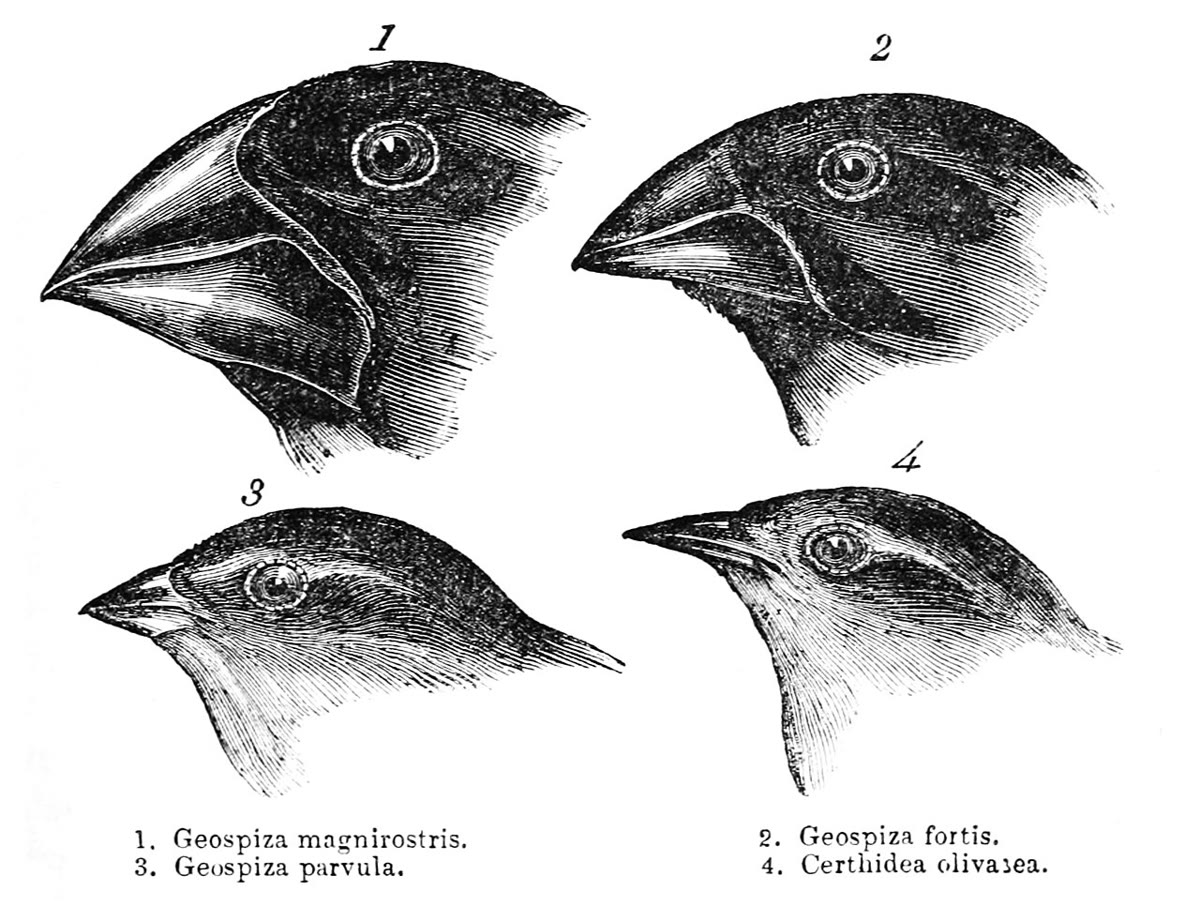
\includegraphics[width=0.44\linewidth]{images/book2/finches-gould.jpg}\hspace{0.04\linewidth}
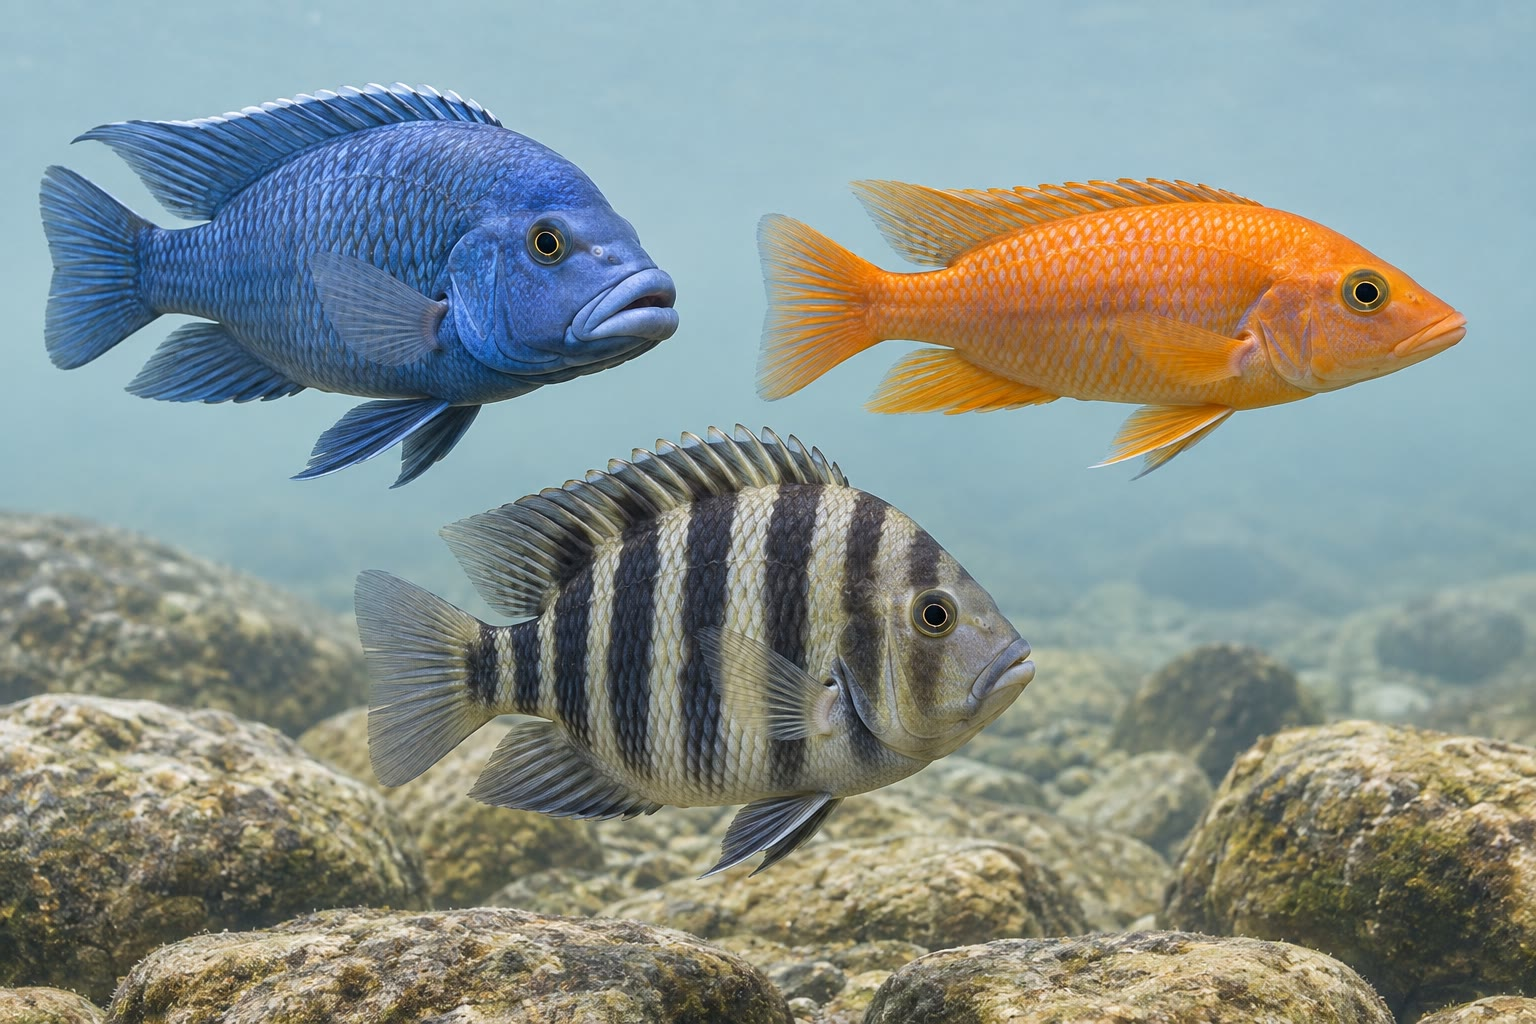
\includegraphics[width=0.44\linewidth]{images/book4/ai/b4-23-cichlids.jpg}

{\small Two radiations. Left: Darwin's finches as drawn by Gould in
1845, one colonist become many, distinguished by their beaks.
Right: cichlids of an African lake, hundreds of species from a few
founders, each with its own mouth and diet.}
\end{omfigure}

\section{Macroevolution: the long view}

\begin{proposition}[Tempo and mode]\label{prop:b2:speciation:tempo}
\index{punctuated equilibrium}\index{gradualism}\index{mass extinction}
Over a few dozen generations the moth changed colour and the finch
its beak; over millions of years the fossil record shows lineages
that hardly change for long stretches and then, in a geological
instant of a few thousand years, are replaced by a distinct
descendant --- \emph{\omterm{prop:b2:speciation:tempo}{punctuated equilibrium}}, which is what
\omterm{prop:b2:speciation:modes}{allopatric speciation} in small peripheral populations followed by
their spread looks like when sampled every hundred thousand years;
and it shows other lineages, the horses among them, that change
gradually across dozens of species. Above the species, the record
is one of turnover: most species last one to ten million years,
the \emph{background extinction} rate is about one species in a
million per year, and five times --- at the end of the Ordovician,
Devonian, Permian (when nine tenths of marine species vanished),
Triassic and Cretaceous --- a \emph{\omterm{prop:b2:speciation:tempo}{mass extinction}} removed most of
what lived within a few hundred thousand years and reset the game,
the survivors radiating into the emptied niches: the mammals into
the dinosaurs' world after the asteroid of 66 million years ago.
Macroevolution is the pattern that the microevolution of this and
the previous chapter, run for a very long time and interrupted by
catastrophe, has drawn.
\end{proposition}

\begin{example}[Rates compared]\label{ex:b2:speciation:rates}
Selection on the finches changed beak depth by \qty{4}{\%} in one
generation; the whole Galápagos radiation, fourteen species from
one founder, took two million years; the difference between a mouse
and an elephant in body size, some $10^{5}$, could be produced by
selection of the finch strength in a few thousand generations ---
and the record shows it took forty million years. The paradox is
resolved by noticing that selection rarely pushes the same way for
long: it reverses with the weather, as it did on Daphne Major the
year after the drought, and \omterm{prop:b2:population-genetics:kinds}{stabilising selection} holds most
lineages where they are. Sustained change is rare, which is why
speciation, which needs it, is slow --- and why, when the world
changes fast, as it does in \cref{ch:b2:global-change}, the
lineages that cannot follow are lost.
\end{example}

\section{Exercises}

\begin{exercise}[$\star$]\label{exo:b2:speciation:1}
State the \omterm{def:b2:speciation:species}{biological species concept} and give three cases in which
it cannot be applied, with the concept used instead.
\end{exercise}

\begin{exercise}[$\star$]\label{exo:b2:speciation:2}
Classify as prezygotic or postzygotic: two frogs breeding in
different months; a mule; a sea urchin sperm that cannot bind
another species' egg; hybrid plants that are vigorous but whose
\omterm{def:b2:angiosperm-reproduction:seed}{seeds} do not germinate; two crickets with different songs.
\end{exercise}

\begin{exercise}[$\star$]\label{exo:b2:speciation:3}
Define allopatric, peripatric, sympatric and \omterm{prop:b2:speciation:modes}{parapatric
speciation}, with an example of each.
\end{exercise}

\begin{exercise}[$\star$]\label{exo:b2:speciation:4}
State the four outcomes of \omterm{thm:b2:speciation:lv}{Lotka--Volterra competition} and the
condition for stable coexistence in words.
\end{exercise}

\begin{exercise}[$\star\star$]\label{exo:b2:speciation:5}
With $K_1 = 1000$, $K_2 = 800$, $\alpha = 0.5$, $\beta = 0.6$,
compute the equilibrium densities and check that each species can
invade the other's carrying capacity.
\end{exercise}

\begin{exercise}[$\star\star$]\label{exo:b2:speciation:6}
With $K_1 = 1000$, $K_2 = 800$, $\alpha = 1.5$, $\beta = 0.3$, which
species wins, and why? What if $\alpha = 1.5$ and $\beta = 1.5$?
\end{exercise}

\begin{exercise}[$\star\star$]\label{exo:b2:speciation:7}
A tetraploid arises in a \omterm{def:b2:meiosis-heredity:meiosis}{diploid} population. Give the chromosome
numbers of its gametes, of a cross with the \omterm{def:b2:meiosis-heredity:meiosis}{diploid}, and of that
hybrid's gametes, and explain why the tetraploid is isolated at
once. Why does it nevertheless usually fail to persist?
\end{exercise}

\begin{exercise}[$\star\star$]\label{exo:b2:speciation:8}
Two populations have each fixed 10 substitutions since they split,
and each pair of new \omterm{def:b2:meiosis-heredity:vocabulary}{alleles} from the two sides is incompatible
with probability $0.01$. Compute the expected number of
incompatibilities now, and after 30 substitutions each. What
does this predict for the relation of isolation to time?
\end{exercise}

\begin{exercise}[$\star\star$]\label{exo:b2:speciation:9}
Compute the width of a \omterm{prop:b2:speciation:reinforcement}{hybrid zone} for dispersal $\sigma =
\qty{2}{km}$ per generation and hybrid disadvantage $s = 0.05$, and
for $\sigma = \qty{0.3}{km}$ and $s = 0.4$. Which zone is more likely
to end in reinforcement, and why?
\end{exercise}

\begin{exercise}[$\star\star\star$]\label{exo:b2:speciation:10}
Two finch species compete for \omterm{def:b2:angiosperm-reproduction:seed}{seeds} with $\alpha = \beta = 0.9$ and
$K_1 = K_2 = 500$. Do they coexist? \omterm{prop:b2:speciation:displacement}{Character displacement} reduces
$\alpha$ and $\beta$ to $0.4$: recompute the equilibrium. Explain in
terms of the isoclines what displacement did.
\end{exercise}

\begin{exercise}[$\star\star\star$]\label{exo:b2:speciation:11}
The Grants found that after the 2004 drought the medium ground
finch's mean beak depth fell by \qty{0.7}{mm} with $h^{2} = 0.7$,
the survivors having been \qty{1}{mm} smaller-beaked than the
population. Check the response with the \omterm{thm:b2:population-genetics:heritability}{breeder's equation}, and
explain why the large ground finch's presence, not the drought
alone, caused the direction of the change.
\end{exercise}

\begin{exercise}[$\star\star\star$]\label{exo:b2:speciation:12}
``Species are made by accident and kept by selection.'' Discuss,
with the two-locus model, reinforcement, and the role of geography.
\end{exercise}

\section{Problem: Two Finches on an Island}

\begin{problem}[{Weekend problem --- a resident finch meets an
invader: their competition analysed on the phase plane, the
displacement of the resident's beak predicted from the breeder's
equation, and the isolation between them measured against a hybrid
zone, ending on the equilibrium densities, the beak's shift, and
the cline width}]
\label{pb:b2:speciation:1}
Resident species 1: $K_1 = 1200$, $r_1 = 0.5$ per year; invader
species 2: $K_2 = 400$. Before displacement $\alpha = 0.9$, $\beta =
0.3$; a drought halves both carrying capacities for one year. Beak
depth of species 1: mean \qty{9.5}{mm}, standard deviation
\qty{0.8}{mm}, $h^{2} = 0.7$. \omterm{prop:b2:speciation:reinforcement}{Hybrid zone} parameters: $\sigma =
\qty{0.5}{km}$, $s = 0.2$.

\medskip
\noindent\textbf{Part I --- The invasion.}
\begin{enumerate}
  \item Write the two isoclines and their intercepts.
  \item Can species 2 invade species 1 at $K_1$? Can species 1
        invade species 2 at $K_2$? Conclude on the outcome.
  \item Compute the equilibrium densities.
  \item Compute $\mathrm{d}N_1/\mathrm{d}t$ at the moment species 2
        arrives with $N_2 = 20$ and $N_1 = 1200$. What does its sign
        mean?
  \item During the drought both $K$ are halved. Recompute the
        equilibrium and say what happens to each species' numbers.
  \item Why is the invader's effect on the resident ($\alpha = 0.9$)
        larger than the resident's on the invader ($\beta = 0.3$)?
\end{enumerate}

\medskip
\noindent\textbf{Part II --- Displacement.}
In the drought the resident individuals with the largest beaks
compete most with the invader and die: the survivors have a mean
beak of \qty{9.0}{mm}.
\begin{enumerate}[resume]
  \item Compute the selection differential and the response.
  \item Give the next generation's mean beak.
  \item After the shift, $\alpha$ falls to $0.5$. Recompute the
        equilibrium (with the original $K$).
  \item Explain what the shift did to species 1's isocline.
  \item If selection of this strength acted every year, how many
        years would it take to shift the beak by \qty{2}{mm}? Why
        does it not?
  \item Compare with the two-million-year age of the radiation and
        comment.
\end{enumerate}

\medskip
\noindent\textbf{Part III --- Isolation.}
The two species can hybridise; hybrids have intermediate beaks and
\omterm{def:b2:population-genetics:fitness}{fitness} $1 - s$.
\begin{enumerate}[resume]
  \item Name the prezygotic barrier that keeps hybridisation rare
        in Darwin's finches, and one postzygotic cost of the
        hybrids.
  \item Compute the width of a \omterm{prop:b2:speciation:reinforcement}{hybrid zone} between them for $\sigma
        = \qty{0.5}{km}$, $s = 0.2$.
  \item The island is \qty{1}{km} across. What does that imply?
  \item Explain how reinforcement would proceed, and what character
        it would act on.
  \item Two populations of the resident on different islands have
        each fixed 15 substitutions since they separated; pairs are
        incompatible with probability $0.005$. Compute the expected
        incompatibilities and say whether they are species.
  \item Would the \omterm{def:b2:speciation:species}{biological species concept}, the morphological
        concept and the phylogenetic concept agree about the two
        island populations? Explain.
\end{enumerate}

\medskip
\noindent\textbf{Part IV --- The long view.}
\begin{enumerate}[resume]
  \item If a species lasts on average 5 million years, what is the
        background extinction rate per species per year? For a
        biota of 10 million species, how many extinctions a year?
  \item The current extinction rate is estimated at 100 to 1000
        times background. How many species a year is that?
  \item A \omterm{prop:b2:speciation:tempo}{mass extinction} removes \qty{75}{\%} of species in
        \num{100000} years. Compare its rate with the present one.
  \item Explain in one sentence why the survivors of a \omterm{prop:b2:speciation:tempo}{mass
        extinction} radiate.
  \item A lineage in the record changes little for 3 million years,
        then is replaced within \num{20000} years by a distinct
        descendant. Name the pattern and give the speciation mode
        that produces it.
  \item Using the finch's \qty{4}{\%} per generation, how many
        generations of sustained selection would double beak depth?
        Why does the fossil record show such changes taking millions
        of years?
  \item State the result: the outcome and equilibrium of the
        competition before and after displacement, the beak's shift
        in one generation, and the \omterm{prop:b2:speciation:reinforcement}{hybrid zone} width.
\end{enumerate}
\end{problem}
